
\section{Background and motivations}
\label{sec:background}

This section introduces the general outlines of the random peer sampling
protocols. Then, it details two state-of-the-art approaches that will be used
later on. Finally, we highlight the motivations of our approach.

\subsection{Random peer sampling}
Random peer sampling protocols (REF) provide each peer with a partial view
$\mathcal{P}$ of the network membership $N$. The partial views are populated
with a uniform distribution of randomly chosen peers. A wide variety of
gossip-based protocols use random peer sampling (e.g. topology management
(REF)). Nonetheless, providing each peer with a uniform random sample relying
solely on local knowledge remains challenging (REF?).  Our Scamplon protocol is
based on two state-of-the-art approaches, namely Scamp and Cyclon.

%% Talk about Cyclon
\begin{asparadesc}
\item [Cyclon]\cite{voulgaris2005cyclon} is a periodic random peer sampling
  protocol which updates its partial view every interval of time. The partial
  view has a fixed-size set at start. In this view, each neighbour is
  associated with an age incremented at each cycle. To update its partial view,
  Cyclon exchanges a subset of its partial view with one of its neighbour
  chosen using the age.  Assuming a well chosen $|\mathcal{P}|$, Cyclon quickly
  converges to a random graph (cf. (REF experiments)) providing desirable
  properties such as robustness (MOAR) etc.  Figure~\ref{fig:cyclonexample}
  depicts the periodic exchanges of Cyclon. We can see that peers only
  communicate in their direct neighbourhood to renew connections.
\end{asparadesc}

\begin{figure}
  \centering
  
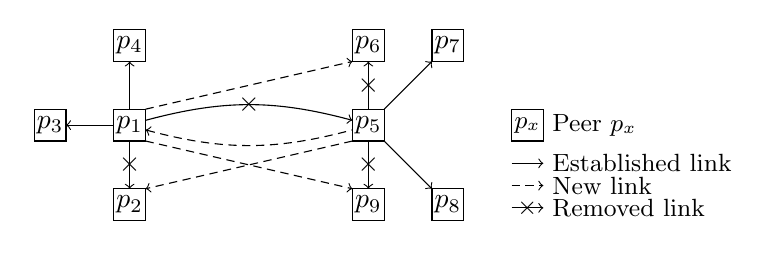
\begin{tikzpicture}[scale=1.15]
  
  \draw[fill=white] (0pt, 0pt) node{$p_1$} +(-5pt,-5pt) rectangle +(5pt,5pt);
  \draw[fill=white] ( 0pt,-25pt) node{$p_2$} +(-5pt,-5pt) rectangle +(5pt,5pt);
  \draw[fill=white] (-25pt,0pt) node{$p_3$} +(-5pt,-5pt) rectangle +(5pt,5pt);
  \draw[fill=white] ( 0pt,25pt) node{$p_4$} +(-5pt,-5pt) rectangle +(5pt,5pt);

  \draw[->] (-5pt, 0pt) -- (-20pt, 0pt); %% p1 -> p2
  \draw[->] ( 0pt, 5pt) -- (  0pt,20pt); %% p1 -> p3
  \draw[->] ( 0pt,-5pt) -- node{$\times$} (  0pt,-20pt); %% p1 -> p4
  
  \begin{scope}[shift={(75pt,0pt)}]
  \draw[fill=white] ( 0pt, 0pt) node{$p_5$} +(-5pt,-5pt) rectangle +(5pt,5pt);
  \draw[fill=white] (0pt,  25pt) node{$p_6$} +(-5pt,-5pt) rectangle +(5pt,5pt);
  \draw[fill=white] ( 25pt,25pt) node{$p_7$} +(-5pt,-5pt) rectangle +(5pt,5pt);
  \draw[fill=white] (25pt,-25pt) node{$p_8$} +(-5pt,-5pt) rectangle +(5pt,5pt);
  \draw[fill=white] (0pt, -25pt) node{$p_9$} +(-5pt,-5pt) rectangle +(5pt,5pt);

  \draw[->] ( 5pt, 5pt) -- ( 20pt, 20pt);
  \draw[->] ( 5pt, -5pt) -- ( 20pt,-20pt);
  \draw[->] ( 0pt, 5pt) -- node{$\times$} ( 0pt,20pt);
  \draw[->] ( 0pt,-5pt) -- node{$\times$} ( 0pt,-20pt);
  \end{scope}
  
  \draw[->, densely dashed] (5pt,5pt) -- (70pt,20pt); 
  \draw[->, densely dashed] (70pt,-5pt) -- (5pt,-20pt);
  \draw[->, densely dashed] ( 5pt,-5pt) -- (70pt,-20pt);
  \draw[->] (5pt, 1.5pt) to[out=15,in=165]
  node{$\times$} (70pt, 1.5pt);
  \draw[<-, densely dashed] (5pt, -1.5pt) to[out=-15,in=-165] (70pt,-1.5pt);

  \small 
  \begin{scope}[shift={(120pt,0pt)}]
    \draw[fill=white](5pt, 0pt)node{$p_x$}+(-5pt,-5pt) rectangle +(5pt,5pt);
    \draw (10pt,0pt) node[anchor=west]{Peer $p_x$};
    \draw[->](0pt, -12pt)--(10pt, -12pt) node[anchor=west]{Established link};
    \draw[->, densely dashed](0pt, -19pt)--(10pt, -19pt)
    node[anchor=west]{New link};
    \draw[->](0pt, -26pt)-- node{$\times$}(10pt, -26pt)
    node[anchor=west]{Removed link};
    
  \end{scope}
  
\end{tikzpicture}
  \caption{\label{fig:cyclonexample}Example of Cyclon's periodic exchange of
    partial views. For simplicity sake, we set $|\mathcal{P}|$ to $3$ and the
    exchanges concern only $2$ neighbours. Furthermore, while the network
    contains $8$ members, we only show the partial views of $p_1$ and $p_5$.
    Peer $p_1$ initiates the view exchange with its oldest neighbour $p_5$,
    giving $\left\{p_1,\,p_4\right\}$. On receipt, Peer $p_5$ establishes the
    connection to $p_1$ and $p_4$ and gives away its connection to
    $\left\{p_7\right\}$.  On receipt of this latter, $p_1$ establishes the
    connection to Peer $p_7$. Altogether, we cut $3$ links to create $3$ other
    links only by using neighbour-to-neighbour interactions.}
\end{figure}

%% Talk about Scamp
\begin{asparadesc}
\item [Scamp]\cite{ganesh2003peer} stands for SCalable Membership
  Protocol. This protocol links each membership event with an appropriate
  reaction.  The most important event is the joining event which creates a
  logarithmically increasing number of connections compared to the total
  network size.  Figure~\ref{fig:scampexample} depicts the joining protocol of
  Scamp. As we can see, the resulting graph is connected. However, the last
  peer $p_1$ only has one neighbour in its partial view, meaning that if $p_4$
  crashes, $p_1$ cannot send messages to the network any more. To avoid that, a
  periodic re-subscription is necessary. This re-subscription mechanism will
  likely add new neighbours in the partial view of the newest peers and
  reorganise the neighbourhood of oldest peer. Just as Cyclon, Scamp converges
  to a random graph and provide their desirable properties.
\end{asparadesc}

\begin{figure}
  \centering
  
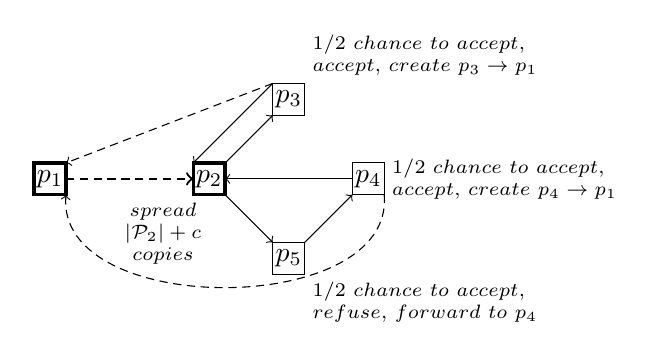
\begin{tikzpicture}[scale=1.15]
  
  \draw[fill=white, very thick] (0pt, 0pt)
  node{$p_1$} +(-5pt,-5pt) rectangle +(5pt,5pt);

  \begin{scope}[shift={(75pt,0pt)}]
  \draw[fill=white, very thick]
  (-25pt, 0pt) node{$p_2$} +(-5pt,-5pt) rectangle +(5pt,5pt);
  \draw[fill=white] (0pt,  25pt) node{$p_3$} +(-5pt,-5pt) rectangle +(5pt,5pt);
  \draw[fill=white] ( 25pt, 0pt) node{$p_4$} +(-5pt,-5pt) rectangle +(5pt,5pt);
  \draw[fill=white] (0pt, -25pt) node{$p_5$} +(-5pt,-5pt) rectangle +(5pt,5pt);


  \draw[->] (-20pt, 5pt) -- (-5pt, 20pt); 
  \draw[->] (-20pt,-5pt) -- (-5pt,-20pt); 
  \draw[->] ( 5pt,-20pt) -- (20pt, -5pt); 
  \draw[->] (20pt,  0pt) -- (-20pt, 0pt); 
  \draw[->] (-5pt, 30pt) -- (-30pt, 5pt); 

  \draw[->, thick, densely dashed] (-70pt, 0pt) -- (-30pt, 0pt); 
  \draw[->, densely dashed] (-5pt, 30pt) -- (-70pt, 5pt); 
  \draw[->, densely dashed] (30pt, -5pt)to[out=-85,in=-95](-70pt,-5pt);

  \scriptsize
  \draw (-25pt,-5pt) node[align=center,anchor=north east]
  {$spread$\\$|\mathcal{P}_2|+c$\\$copies$};
  \draw (5pt,-30pt) node[align=left,anchor=north west]
  {$1/2$ $chance$ $to$ $accept,$\\$refuse,$ $forward$ $to$ $p_4$};
  \draw (5pt, 30pt) node[align=left,anchor=south west]
  {$1/2$ $chance$ $to$ $accept,$\\$accept,$ $create$ $p_3 \rightarrow p_1$};
  \draw (30pt, 0pt) node[align=left,anchor=west]
  {$1/2$ $chance$ $to$ $accept,$\\$accept,$ $create$ $p_4 \rightarrow p_1$};
  \end{scope}
  
%%  \small
%%  \begin{scope}[shift={(130pt,0pt)}]
%%    \draw[fill=white](5pt, 0pt)node{$p_x$}+(-5pt,-5pt) rectangle +(5pt,5pt);
%%    \draw (10pt,0pt) node[anchor=west]{Peer $p_x$};
%%    \draw[->](0pt, -12pt)--(10pt, -12pt) node[anchor=west]{Established link};
%%    \draw[->, densely dashed](0pt, -19pt)--(10pt, -19pt)
%%    node[anchor=west]{New link};
%%    
%%  \end{scope}
  
\end{tikzpicture}
  \caption{\label{fig:scampexample} Scamp's joining protocol on a small
    network. Peer $p_1$ wants to join $p_4$'s network composed of $p_2$,
    $p_3$, $p_4$, and $p_5$. Peer $p_1$ establishes a connection to $p_4$. Then
    $p_4$ copies $|\mathcal{P}|$-times the new subscription and sends one to
    each neighbour. To handle possible failures, $c$ additional copies (here
    $0$ for simplicity sake), are sent to random neighbours. Then, each peer
    has a probability of $1\over{|\mathcal{P}|+1}$ to accept the forwarded
    subscription, hence, to establish a connection to reach $p_1$. Otherwise,
    the peer forwards it to another peer in $\mathcal{P}$ at random. Here,
    $p_3$ accepts the subscription, $p_2$ forwards it to $p5$, and the latter
    accepts it. The resulting graph is connected.}
\end{figure}

\subsection{Motivations}
In this paper, we do not restrict ourselves to one-way connections. We also
study the effect of three-way handshake connection set-up. The connection
establishment using such set-up forces a round trip negotiation much more
costly and subject to failure. In this context, each connection matters. Hence,
we cannot afford oversized partial views. Consequently, one would be tempted to
use Scamp. However the subscription mechanism can create connections several
hops away from the origin. Each of these hops is an opportunity of failure
(cf. Fig~\ref{fig:failureexample}).

Let $P_f$ the probability of either the peer or the link between the latter and
the next peer crashes/disconnects when it holds the subscription, without
possible recovery. Let $P_E$ the probability that a connection establishment
cannot be completed. Without handshake, $P_E$ is straightforward:
\begin{equation} P_{E,\,1way}^{Cyclon}=1-(1- P_f)^2 \end{equation}
\begin{equation} P_{E,\,1way}^{Scamp}=1-(1- P_f)^k \end{equation} where $k$ is
the number of hops before the acceptance of the subscription. On the other
hand, in the handshaking context, the subscription must travel back to its
origin in order to be completed. As consequence, when a subscription travels
through a peer or a link, they are not allowed to fail until the subscription
travels back. Thus, we have (TO DOUBLE CHECK):
\begin{equation} P_{E,\,3way}^{Cyclon}=1-(1- P_f)^6\end{equation}.
\begin{align} P_{E,\,3way}^{Scamp} &=1 - ((1-P_f)^{2k} (1-P_f)^{2(k-1)}
                                     \ldots (1-P_f)^2) \\
                                   &=1-(1-P_f)^{k^2+k}
\end{align}
From these analysis, it is worth noting that while Cyclon remains at a same
order of magnitude in both cases, Scamp is dramatically impacted. To sustain
these theoretical analysis, we conducted series of experiments to highlight the
differences between the contexts and the influence of failures on convergence
speed (INSERT GRAPH).

\begin{figure}
  \centering
  
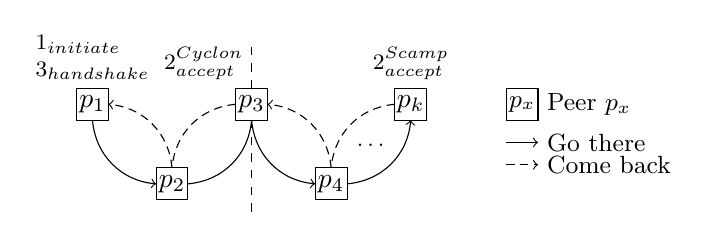
\begin{tikzpicture}[scale=1.15]

  \footnotesize
  \draw (0pt,5pt)node[align=left,anchor=south]{$1_{initiate}$\\
    $3_{handshake}$};
  \draw (50pt, 5pt)node[anchor=south east]{$2_{accept}^{Cyclon}$};
  \draw (100pt,5pt)node[anchor=south]{$2_{accept}^{Scamp}$};
  \draw (88pt, -13pt)node{\ldots};

  \draw[dashed](50pt,-5pt)--(50pt,-35pt);
  \draw[dashed](50pt, 5pt)--(50pt, 20pt);

  \normalsize
  \draw[fill=white] (0pt, 0pt) node{$p_1$} +(-5pt,-5pt) rectangle +(5pt,5pt);
  \draw[fill=white] (25pt,-25pt) node{$p_2$} +(-5pt,-5pt) rectangle +(5pt,5pt);
  \draw[fill=white] (50pt, 0pt) node{$p_3$} +(-5pt,-5pt) rectangle +(5pt,5pt);
  \draw[fill=white] (75pt,-25pt) node{$p_4$} +(-5pt,-5pt) rectangle +(5pt,5pt);
  \draw[fill=white] (100pt, 0pt) node{$p_k$} +(-5pt,-5pt) rectangle +(5pt,5pt);


  \draw[->] ( 0pt,-5pt) to[out=-85,in=175] (20pt,-25pt);
  \draw[->, densely dashed] (25pt, -20pt) to[out=95,in=-5] ( 5pt, 0pt);
  \draw     ( 30pt, -25pt) to[out=5,in=-95] (50pt,-5pt);
  \draw[densely dashed] ( 45pt, 0pt) to[out=185,in=85] (25pt, -20pt);
  \draw[->] (50pt, -5pt) to[out=-85,in=175] (70pt,-25pt);
  \draw[->, densely dashed] (75pt, -20pt) to[out=95,in=-5] (55pt,0pt);
  \draw[->] (80pt, -25pt) to[out=5pt,in=-95] (100pt,-5pt);
  \draw[densely dashed] (95pt, 0pt) to[out=185,in=85] (75pt, -20pt);
%%  \draw[->, densely dashed] (-70pt, 0pt) -- (-30pt, 0pt); %% u1 -> u4
%%  \draw[->, densely dashed] (-5pt, 30pt) -- (-70pt, 5pt); %% u3 -> u1
%%  \draw[->, densely dashed] (30pt, -5pt) to[out=-85,in=-95](-70pt,-5pt);%%u5 u1

  \small 
  \begin{scope}[shift={(130pt,0pt)}]
    \draw[fill=white](5pt, 0pt)node{$p_x$}+(-5pt,-5pt) rectangle +(5pt,5pt);
    \draw (10pt,0pt) node[anchor=west]{Peer $p_x$};
    \draw[->](0pt, -12pt)--(10pt, -12pt) node[anchor=west]{Go there};
    \draw[->, densely dashed](0pt, -19pt)--(10pt, -19pt)
    node[anchor=west]{Come back};    
  \end{scope}
  
\end{tikzpicture}
  \caption{\label{fig:failureexample}Handshaking differences of Cyclon and
    Scamp. While subscriptions travel from $p_1$ to $p_3$ using one
    intermediate in Cyclon, the subscriptions travel from $p_1$ to $p_k$ in
    Scamp. This difference change the complexity of the two approaches. In
    particular, the failure probability is much more important in
    Scamp. Indeed, links and peers, once employed, must be kept alive until the
    subscriptions travel back. Otherwise, the handshaking is not complete.}
\end{figure}

To summarise, we would like the best of the aforementioned approaches: a random
peer sampling protocol providing a logarithmically growing partial view size
compared to the network membership, using neighbour-to-neighbour interactions
to establish connections, quickly converging to a random network.

%%% Local Variables:
%%% mode: latex
%%% TeX-master: "../paper"
%%% End:
